\begin{problem}{Minimax and Alpha-Beta Pruning}
Note: Triangle nodes pointing up refer to max nodes, and triangle nodes pointing down refer to min nodes.

\begin{center}
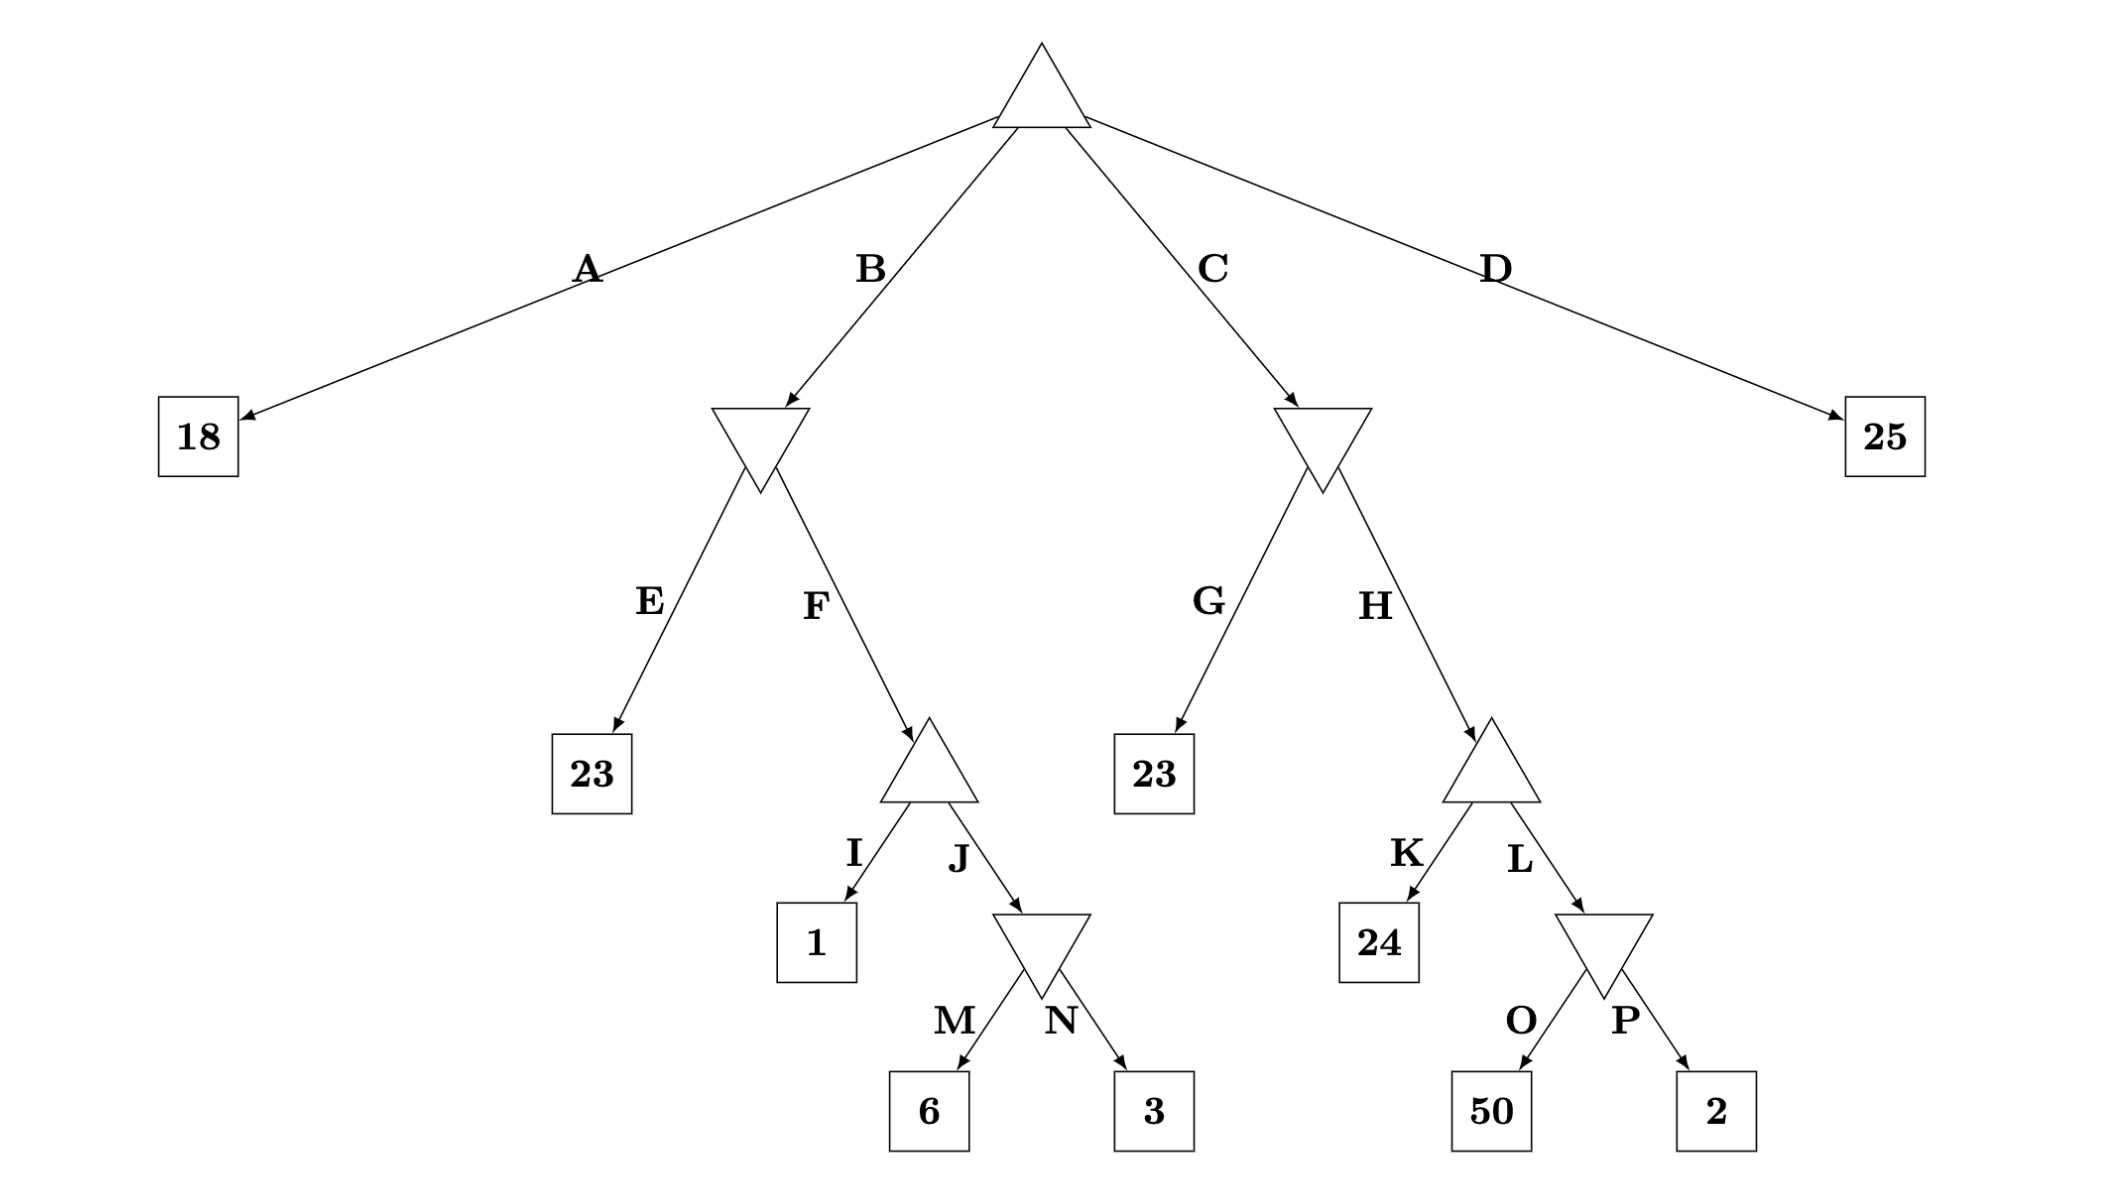
\includegraphics[width=400 pt]{figures/Minimax-and-AlphaBeta-q6.png}
\end{center}

\begin{question}[1]
What is the minimax value of the root?

\solutionspace{1.2cm}{1.5cm}{Answer:}{ \SixA}
\end{question}

\begin{question}[2]
What are the minimax value for the minimizer nodes at level 2 (assuming the root node is at level 1)?
\begin{subquestion}[1]

\solutionspace{1.2cm}{2cm}{Answer B:}{ \SixBi}
\end{subquestion}
\qquad
\begin{subquestion}[1]

\solutionspace{1.2cm}{2cm}{Answer C:}{ \SixBii}
\end{subquestion}
\end{question}

\begin{question}[4]
Assuming children are visited in left-to-right order, which branches (letters)  would be pruned by alpha-beta pruning?

NOTE: select the top most branch that can be pruned. For example, if branch B is pruned, then we know E and F are both pruned as well. However, in this case, only select B as your answer.

\solutionspace{1.2cm}{4cm}{Answer:}{ \SixC}

\end{question}

\begin{question}[4]
Which of the below orderings would result in the most pruning (select all that apply)? Assume all other nodes are visited in left-to-right order, except for children of the root. For example, if you believe left-to-right order would result in the most pruning, you should select A,B,C,D.

\solution{\emptysquare}{\SixDi} A,B,C,D
\qquad
\solution{\emptysquare}{\SixDii} C,D,A,B
\qquad
\solution{\emptysquare}{\SixDiii} D,A,B,C
\qquad
\solution{\emptysquare}{\SixDiv} D,A,C,B
\qquad
\solution{\emptysquare}{\SixDv} B,D,A,C

\end{question}
\end{problem}